\section{Application}
%\KZ{Add another pic side-by-side that shows the front page of iWen and also a pic that
%shows the context of this question, to convince ppl that this is a real app.
%Also tell them how long this app has been deployed, where they can download it and what is the
%lastest version.}
In this section, we demonstrate how the proposed framework is deployed in real-world application. The  most suitable scenario to implement our distractor generation system is AI-assisted education, especially in language learning. Our framework has been successfully deployed in an English learning and reading app called iWen. iWen has been released to the market since 2018 and is being active developed. The latest version is 1.5.3 for iOS and 1.0.40 for Android. It can be downloaded from Apple AppStore and 
all Android application markets. iWen provides massive volume of English reading materials 
such as fictions and non-fictions, and up-to-the-minute news for users to improve their 
vocabulary and reading skill. At the end of each chapter of book or news, it will generate 
several multiple-choice questions to assess how well users comprehend the content. 
In the implementation, after locating question-worthy context as question body and keyword as 
correct answer, our CSG+DS distractor generation framework is then applied to 
automatically generate distractive options that will be put together with correct answer 
to form a complete multiple-choice question.

An overview of iWen and application of our 
distractor generation framework is shown in \figref{fig:app}, where the user 
select \textit{signed} as the answer after reading the news:
\begin{figure*}[t!]
	 	\centering
 		\scalebox{2.1}{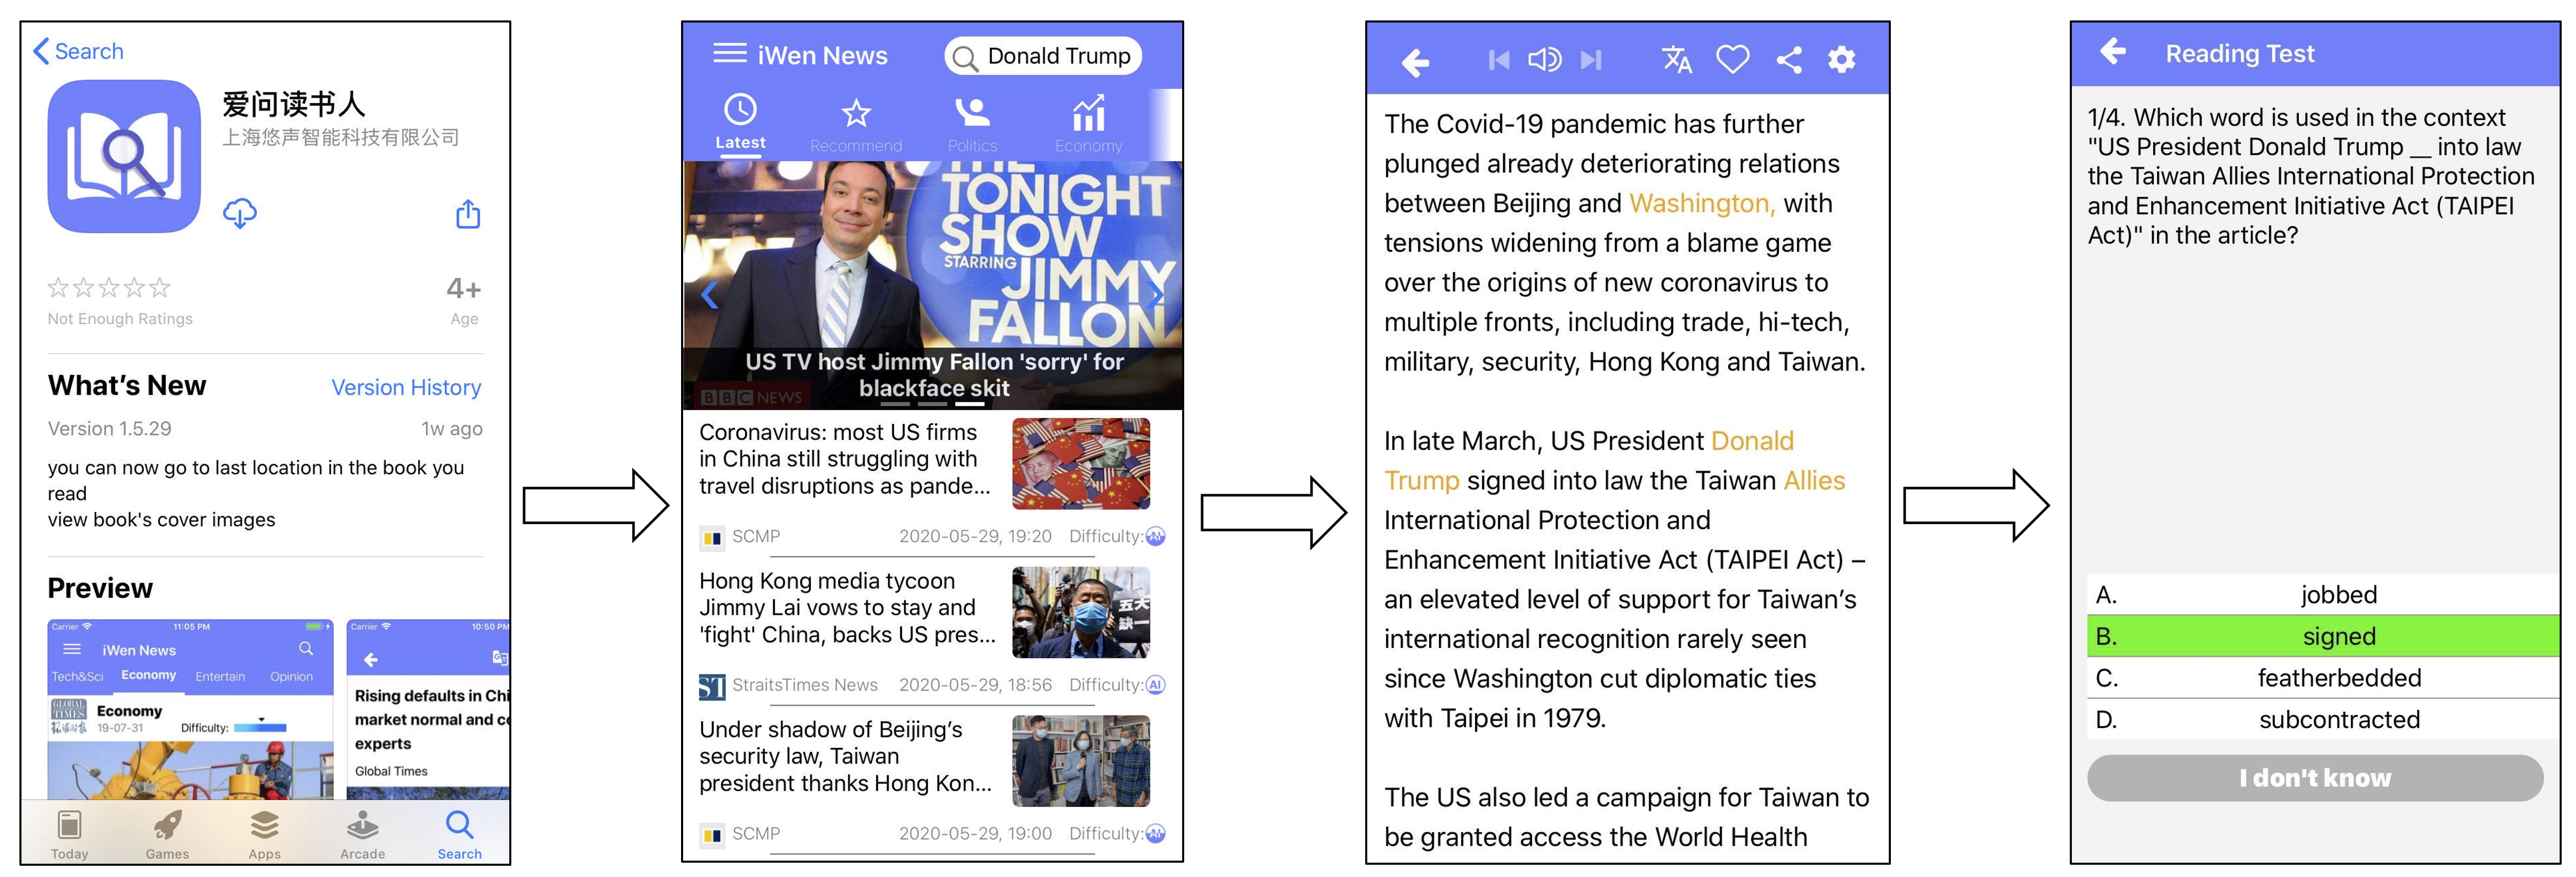
\includegraphics[width=1.0\columnwidth]{figure/iwen.jpg}}
 		\caption{The mobile app iWen in which the proposed distractor generation framework is 
deployed. The left-most picture shows iWen in the Chinese AppStore. 
The right-most screenshot shows one generated MCQ given the news context in 
the previous screenshot.}
 		\label{fig:app}
\end{figure*}
The ideal distractors in MCQs are required to be plausible and reliable to fully test 
the users, which is to a large extent satisfied by our proposed framework. Recent statistics from iWen shows that a user may take the quiz from either books or news 9.4 times per day on average and the chances of users making an incorrect
answer is about 42\%, which validates the effectiveness of our CSG+DS 
framework in practical use.
%\KZ{Give some stats from our app's monitor to show how frequently the quiz feature is used,
%whether the distractors are good according to some implicit feedback from the iWen users.
%This will be very useful, more convincing than just saying that is been deplayed for 2 years.}
